\documentclass[compress, 8pt]{beamer}
% \documentclass[handout, 8pt]{beamer}
\usepackage[utf8]{inputenc}

% Notes to self: \nts[color option]{text that is a note}
\newif\ifshowcomments
% \showcommentstrue % uncomment to show
\input{preambleB}

%%%%%%%%%%%%%%%%%%%%%%%%%%%%%%%%%%%%%%%%%%%%%%%%%%%%%%%%%%%%%%%%%%%%%%%%%%%%%%
% Paths to figures
\usepackage{subcaption}

% Avoid a warning on mac; can introduce a warning (and maybe a break) on windows
% \usepackage{etex}
% Avoid a warning
\let\Tiny=\tiny

%Information to be included in the title page:
\title{Conditional Expectation}
\subtitle{ECON726}
\author[]{Tara Sullivan}
\institute{
Tara Sullivan \\
\textit{tara.sullivan55@login.cuny.edu}
}
\date{
\today
\nts{\\
\medskip
Notes/comments are in gray and will be excluded from the presentation.
}
}

% plot graphs with pgfplots
\usepackage{pgfplots}
\pgfplotsset{compat=newest}
\usepgfplotslibrary{groupplots}
\usepgfplotslibrary{dateplot}
\pgfplotsset{compat=newest,
    every axis/.style={
        axis y line*=left,
        axis x line*=bottom,
        % allows for multi-line legend entries
        legend style={cells={align=left}},
        % allows for multi-line titles
        title style={align=center},
    },
}

% For animations using underbrace 
% Source: https://tex.stackexchange.com/a/565866
\usepackage{xparse, letltxmacro}
\LetLtxMacro{\oldunderbrace}{\underbrace}
\DeclareDocumentCommand{\underbrace}{d<> m e{_}}{%
  \IfValueTF{#1}{% IF <overlay-specification> given
    % using global onlside flag, cf. p82 beamer manual v3.59
    \oldunderbrace{#2\onslide<#1>}_{#3}\onslide%
  }{% ELSE
    \oldunderbrace{#2}_{#3}
  }%
}%

%%%%%%%%%%%%%%%%%%%%%%%%%%%%%%%%%%%%%%%%%%%%%%%%%%%%%%%%%%%%%%%%%%%%%%%%%%%%%%%%
\begin{document}    
%\beamertemplatenavigationsymbolsempty


%%%%%%%%%%%%%%%%%%%%%%%%%%%%%%%%%%%%%%%%%%%%%%%%%%%%%%%%%%%%%%%%%%%%%%%%%%%%%%%%
\begin{frame}
\titlepage
% \tikzset{external/figure name={intro_}}
\end{frame}

\begin{frame}{Housekeeping}


\begin{itemize}
    \item Please check any comments on your homework
    \item Homework this week: submit 1-2 possible papers for your project. Be ambitious and creative!
    \item Read MHE 3.1 (skim 3.1.3 if it's difficult) and 3.2 (skim 3.2.3)
    \begin{itemize}
        \item Optional additional reading: Chapter 1 of the Causal ML book (more advanced and ML-focused) \url{https://chapters.causalml-book.org/CausalML_chap_1.pdf}
    \end{itemize}
\end{itemize}

Agenda:
\begin{itemize}
    \item Discuss resource for looking for papers %: \url{https://www.aeaweb.org/journals}
    \item Review slides
    \item Review google notebooks for python intro: \url{https://github.com/tara-sullivan/econ726-notebooks}
    \item Time permitting: properties of the CEF (MHE 3.1.1.)
    % \item Time permitting: stats review: \url{https://matheusfacure.github.io/python-causality-handbook/03-Stats-Review-The-Most-Dangerous-Equation.html}
\end{itemize}

\end{frame}

%%%%%%%%%%%%%%%%%%%%%%%%%%%%%%%%%%%%%%%%%%%%%%%%%%%%%%%%%%%%%%%%%%%%%%%%%%%%%%%
\miniframesoff
\begin{frame}{Outline}
    \tableofcontents
\end{frame}
\miniframeson



%%%%%%%%%%%%%%%%%%%%%%%%%%%%%%%%%%%%%%%%%%%%%%%%%%%%%%%%%%%%%%%%%%%%%%%%%%%%%%%%
\section[Intro]{Introduction}

%%%%%%%%%%%%%%%%%%%%%%%%%%%%%%%%%%%%%%%%%%%%%%%%%%%%%%%%%%%%%%%%%%%%%%%%%%%%%%%%
\begin{frame}{Probability cheat sheet}

Probabilities of two variables, $X$ and $Y$:
\begin{table}
\begin{tabular}{ll}
    $\PP (X, Y)$ &: joint \\
    $\PP (X \vert Y)$ &: conditional \\
    $\PP (X)$ &: unconditional (marginal)
\end{tabular}
\end{table}
Rules:
\begin{table}
\begin{tabular}{lll}
&Unconditional &Conditional \\
\hline
Product Rule 
& $\PP (X, Y) = \PP (X) \PP (Y \vert X)$ 
& $\PP (X, Y \vert E) = \PP(X \vert E) \PP (Y \vert X, E)$ \\
Bayes Rule 
& $\PP (X \vert Y) = \frac{\PP(Y \vert X) \PP(X)}{\PP (Y)}$
& $\PP (X \vert Y, E) = \frac{\PP (Y \vert X, E) \PP(X \vert E)}{\PP(Y \vert E)}$
\\
Marginalization 
& $\PP(X) = \sum_j \PP(X, Y=y_j)$
& $\PP(X \vert E) = \sum_j \PP(X, Y=y_j, \vert E)$
\\
\hline
Independence
& $\PP(X, Y) = \PP(X)\PP(Y)$
& $\PP(X, Y \vert E) = \PP (X \vert E) \PP(Y \vert E)$ \\
& $\implies \PP(X \vert Y) = \PP(X)$
& $\implies \PP(X \vert Y, E) = \PP(X \vert E)$ \\
& $\implies \PP(Y \vert X) = \PP(Y)$
& $\implies\PP(Y \vert X, E) = \PP(Y \vert E)$ \\
\end{tabular}
\end{table}

\end{frame}



%%%%%%%%%%%%%%%%%%%%%%%%%%%%%%%%%%%%%%%%%%%%%%%%%%%%%%%%%%%%%%%%%%%%%%%%%%%%%%%%
\section{Expectation and variance}
\miniframesoff
\begin{frame}
    \tableofcontents[currentsection]
\end{frame}
\miniframeson
%%%%%%%%%%%%%%%%%%%%%%%%%%%%%%%%%%%%%%%%%%%%%%%%%%%%%%%%%%%%%%%%%%%%%%%%%%%%%%%

\begin{frame}{Random variables}


% \vspace{2ex}
Example: Suppose we flip two coins and count the number of heads:
\begin{table}
\begin{tabular}{llc}
Flip 1 &Flip 2  &Final count ($X$) \\
\hline
Heads   &Heads  &2 \\
Heads   &Tails  &1 \\
Tails   &Heads  &1 \\
Tails   &Tails  &0 
\end{tabular}
\end{table}

We can define our random variable $X$ over it's possible outcomes, $\{0, 1, 2\}$:
\begin{table}
\begin{tabular}{cl}
$X$ &$\PP (X = x)$ \\
\hline
0 & $\PP (X = 0) = \frac{1}{4}$\\
1 &$\PP (X = 1) = \frac{1}{2}$\\
2 &$\PP (X = 2) = \frac{1}{4}$\\
\end{tabular}
\end{table}

We can describe the probability of $X$ using the function $p_X(x)$, its \textbf{probability mass function}, \textbf{PMF} (sometimes called the \textbf{discrete probability density function}, or \textbf{PDF}).
\begin{equation*}
    p_X(x) = \begin{cases}
    \frac{1}{4} &\text{if } x = 0 \\
    \frac{1}{2} &\text{if }x=1 \\
    \frac{1}{4} &\text{if }x=2
    \end{cases}
\end{equation*}


% $\PP\left( \frac{1}{2} \right)$ 
% $\PP\left( \frac{1}{2} \right)$

\end{frame}

%%%%%%%%%%%%%%%%%%%%%%%%%%%%%%%%%%%%%%%%%%%%%%%%%%%%%%%%%%%%%%%%%%%%%%%%%%%%%%%%
\begin{frame}{Discrete probability mass function (PMF)}


The PMF can be described graphically: 
\begin{figure}
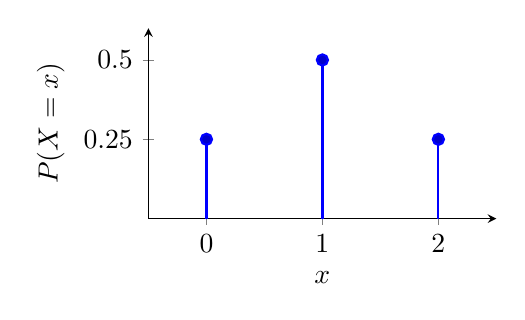
\begin{tikzpicture}
  \begin{axis}[
    ymin=0, ymax=0.6,
    xmin=-0.5, xmax=2.5,
    xtick={0,1,2},
    ytick={0.25,0.5},
    axis lines=left,
    width=6cm,
    height=4cm,
    xlabel={$x$},
    ylabel={$P(X = x)$},
    samples=3,
    domain=0:2,
    % enlargelimits=0.1,
    every axis plot/.append style={ultra thick}
  ]
  
  % Vertical lines
  \addplot+[ycomb, mark=*, blue, thick] coordinates {
    (0, 0.25)
    (1, 0.5)
    (2, 0.25)
  };

  \end{axis}
\end{tikzpicture}
\end{figure}


\end{frame}

%%%%%%%%%%%%%%%%%%%%%%%%%%%%%%%%%%%%%%%%%%%%%%%%%%%%%%%%%%%%%%%%%%%%%%%%%%%%%%%%
\begin{frame}{Expected value}

The expected value of a random variable is its average variable, where the average is weighted according to the probability distribution. 
\begin{itemize}
    \item It is a measure of centrality
    \item ``By weighting the values of the random variable according to the probability distribution, we hope to obtain a number that summarizes a typical or expected value of an observation of the random variable'' (Casella and Berger, pg 55)
    \item $\EE [X]$ is as good a guess at the value of $X$ for a random observation
    \item The expected value is the \textbf{mean} of the possible values of a random variable, weighted by the probability of those outcomes
\end{itemize}


\end{frame}

%%%%%%%%%%%%%%%%%%%%%%%%%%%%%%%%%%%%%%%%%%%%%%%%%%%%%%%%%%%%%%%%%%%%%%%%%%%%%%%%
\begin{frame}{Expected value}

For a discrete random variable that takes on real values $(x_1, x_2, \dots, x_n)$, we can define the mean or \textbf{expected value} as:
\begin{equation*}
\EE [X] = \sum_{i=1}^n x_i \cdot \PP (X = x_i)   
\end{equation*}


In our example where we count the number of heads in two flipped coins, the mean number of heads is: 
\begin{align*}
    \EE [X] &= \sum_{i=0}^2 x_i \PP (X = x_i) \\
    &= 0 \cdot \PP (X = 0) + 1 \cdot \PP (X = 1) + 2 \cdot \PP (X = 2) \\
    &= 0 \cdot \frac{1}{4} + 1 \cdot \frac{1}{2} + 2 \cdot \frac{1}{4} \\
    &= 0 + \frac{1}{2} + \frac{1}{2} \\
    &= 1
\end{align*}
\end{frame}


%%%%%%%%%%%%%%%%%%%%%%%%%%%%%%%%%%%%%%%%%%%%%%%%%%%%%%%%%%%%%%%%%%%%%%%%%%%%%%%%
\begin{frame}{Expected value examples - discrete}

% \textbf{Discrete example:} Let $X$ be the outcome of a fair die. Then the expected value of $X$ is:
% \begin{align*}
%     \mu = \EE [X] =& \sum_{i=1}^6 x_i \PP (X = x_i) \\
%     =& 1 \cdot \frac{1}{6} + 2 \cdot \frac{1}{6} + 3 \cdot \frac{1}{6} + 4 \cdot \frac{1}{6} + 5 \cdot \frac{1}{6} + 6 \cdot \frac{1}{6} \\
%     =& \frac{1}{6} (1 + 2 + 3 + 4 + 5 + 6) \\
%     =& \frac{1}{6} \cdot 21 \\
%     =& \frac{7}{2} = 3.5
% \end{align*}
Suppose the population of interest is eight students in a class. Their grades are:
\begin{equation*}
    2, 4, 4, 4, 5, 5, 7, 9
\end{equation*}
$X$ is the grade of a random student selected from the class. Then:
\begin{align*}
    \mu = \EE [X] &= \sum_{x_i \in\{2, 4, 5, 7, 9\}} x_i \PP (X = x_i) \\
    &= 2 \cdot \frac{1}{8} + 4 \cdot \frac{3}{8} + 5 \cdot \frac{2}{8} + 7 \cdot \frac{1}{8} + 9 \cdot \frac{1}{8} \\
    &= \frac{2 + 12 + 10 + 7 + 9}{8} \\
    =& \frac{40}{8} = 5
\end{align*}
Note you can calculate this value using the arithmetic mean: 
\begin{equation*}
    \mu = \EE [X] = \frac{2 + 4+4+4+5+5+7+9}{8} = \frac{40}{8} = 5
\end{equation*}

\end{frame}


%%%%%%%%%%%%%%%%%%%%%%%%%%%%%%%%%%%%%%%%%%%%%%%%%%%%%%%%%%%%%%%%%%%%%%%%%%%%%%%%
\begin{frame}{Expected value - continuous}

For a continuous random variable, the expected value is given by:
\begin{equation*}
    \EE [X] = \int_{-\infty}^\infty x f_X (x) dx
\end{equation*} 
We won't make you do calculus in this class! But you should be aware of what the integral looks like. 

\begin{figure}
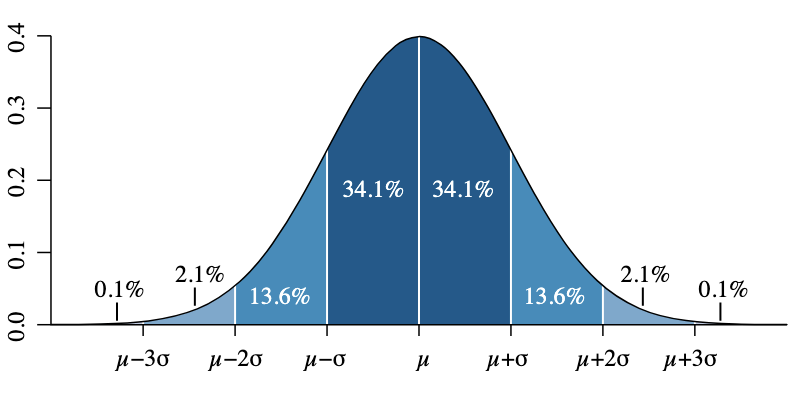
\includegraphics[scale=0.6]{img/normal_distribution.png}
\end{figure}

\end{frame}

%%%%%%%%%%%%%%%%%%%%%%%%%%%%%%%%%%%%%%%%%%%%%%%%%%%%%%%%%%%%%%%%%%%%%%%%%%%%%%%%
\begin{frame}{Expected value of a function}

For any function $g$ and random variable $X$:
\begin{equation*}
\EE [g(X)] = \sum_{i=1}^n g(x_i) \cdot \PP (X = x_i)   
\end{equation*}
Suppose you have a discrete random variable $X$ with the following distribution:
\begin{align*}
    \PP(X = 1) &= 0.5 \\
    \PP (X=2) &= 0.5
\end{align*}
Find the expected value of $X^2$:
\begin{align*}
    \EE[g(X)] = \EE[X^2] &= \sum_x g(x) \PP(X = x) \\
    &= 1^2 \cdot \PP(X = 1) + 2^2 \cdot \PP(X = 2) \\
    &= 1 \cdot 0.5 + 4 \cdot 0.5 \\
    &= 2.5
\end{align*}

\end{frame}


%%%%%%%%%%%%%%%%%%%%%%%%%%%%%%%%%%%%%%%%%%%%%%%%%%%%%%%%%%%%%%%%%%%%%%%%%%%%%%%%
\begin{frame}{Variance and standard deviation}

Variance is the expected value of the squared deviation from the mean:
\begin{equation*}
    \sigma^2 = \Var{X} = \EE [(X - \mu)^2]
\end{equation*}
This gives a measure of the degree of spread of a distribution around its mean. 
\begin{itemize}
    \item Larger values of $\sigma^2$ imply greater dispersion around the mean
\end{itemize}

\vspace{3ex}
\textbf{Standard deviation} is the square root of the variance:
\begin{equation*}
    \sigma = \sqrt{\sigma^2} = \sqrt{\EE \left[ (X - \mu)^2 \right]} 
\end{equation*}

\end{frame}

%%%%%%%%%%%%%%%%%%%%%%%%%%%%%%%%%%%%%%%%%%%%%%%%%%%%%%%%%%%%%%%%%%%%%%%%%%%%%%%%
\begin{frame}{Example: grades of eight students}

Suppose the population of interest is eight students in a class. Their grades are:
\begin{equation*}
    2, 4, 4, 4, 5, 5, 7, 9
\end{equation*}
The mean $\EE [X]$ of their grades equals:
\begin{equation*}
    \mu = \EE [X] = \frac{2 + 4+4+4+5+5+7+9}{8} = \frac{40}{8} = 5
\end{equation*}
Calculate the deviation of each data point:
\begin{align*}
    (2-5)^2 &= (-3)^2 = 9     &(5-5)^2 &= 0^2 = 0 \\
    (4-5)^2 &= (-1)^2 = 1     &(5-5)^2 &= 0^2 = 0 \\
    (4-5)^2 &= (-1)^2 = 1     &(7-5)^2 &= 2^2 = 4 \\
    (4-5)^2 &= (-1)^2 = 1     &(9-5)^2 &= 4^2 = 16
\end{align*}
The variance is the average of these values:
\begin{equation*}
    \sigma^2 = \frac{9+1+1+1+0+0+4+16}{8} = \frac{32}{4}
\end{equation*}
The standard deviation is the square root of the variance:
\begin{equation*}
    \sigma = \sqrt{4} = 2
\end{equation*}

\end{frame}


%%%%%%%%%%%%%%%%%%%%%%%%%%%%%%%%%%%%%%%%%%%%%%%%%%%%%%%%%%%%%%%%%%%%%%%%%%%%%%%%
\begin{frame}{Data}

We often talk about collections of random variables ($X_1, X_2, \dots, X_n$) that are \textbf{independent and identically distributed} (or \textbf{iid}).
\begin{itemize}
    \item The variables each have the same marginal distribution
    \item The variables are all mutually independent
    \begin{itemize}
        \item The occurrence of $X_i$ doesn't impact the occurrence of $X_j$ for all $i$ and $j$
        \item $\PP(X_i \vert X_j = x) = \PP (X_i)$
    \end{itemize}
\end{itemize}
$X_1, X_2, \dots, X_n$ can be referred to as a \textbf{random sample}, and their common marginal distributions are referred to as the \textbf{population} from which the sample is drawn

\end{frame}

%%%%%%%%%%%%%%%%%%%%%%%%%%%%%%%%%%%%%%%%%%%%%%%%%%%%%%%%%%%%%%%%%%%%%%%%%%%%%%%%
\begin{frame}{Sample mean and variance}

The sample mean of a random sample $X_1, \dots, X_n$ is given by:
\begin{equation*}
    \bar{X}_n = \frac{1}{n} \sum_{i=1}^n X_i
\end{equation*}
The sample variance is given by:
\begin{equation*}
    S_n^2 = \frac{1}{n - 1}^n \sum_{i=1} (X_i - \bar{X}_n)^2
\end{equation*}
The sample standard deviation is given by:
\begin{equation*}
    S_n = \sqrt{S_n^2}
\end{equation*}
Note that these are simply sample analogues of the population characteristics we discussed before.


\end{frame}

%%%%%%%%%%%%%%%%%%%%%%%%%%%%%%%%%%%%%%%%%%%%%%%%%%%%%%%%%%%%%%%%%%%%%%%%%%%%%%%%
\begin{frame}{Sample mean and variance (cont.)}

Let $X_1, \dots, X_n$ be iid with common expected value $\EE [X_i] = \mu$ and common variance $\Var{X_i} = \sigma^2$. Then the following holds:
\begin{align*}
    \EE [\bar{X}_n] &= \mu \\
    \Var{\bar{X}_n} &= \frac{\sigma^2}{n} \\
    \EE [S_n^2] &= \sigma^2
\end{align*}

\end{frame}

%%%%%%%%%%%%%%%%%%%%%%%%%%%%%%%%%%%%%%%%%%%%%%%%%%%%%%%%%%%%%%%%%%%%%%%%%%%%%%%%
\section{Covariance and correlation}
\miniframesoff
\begin{frame}
    \tableofcontents[currentsection]
\end{frame}
\miniframeson
%%%%%%%%%%%%%%%%%%%%%%%%%%%%%%%%%%%%%%%%%%%%%%%%%%%%%%%%%%%%%%%%%%%%%%%%%%%%%%%


%%%%%%%%%%%%%%%%%%%%%%%%%%%%%%%%%%%%%%%%%%%%%%%%%%%%%%%%%%%%%%%%%%%%%%%%%%%%%%%%
\begin{frame}{Covariance and Correlation}

So far we've described absence or presence of a relationship between two random variables in terms of independence or non-independence
\begin{itemize}
    \item Now we want to measure the strength of a relationship between two variables
    \item Example: $X$ is weight of a person, $Y$ is the height of a person; clearly these variables are related in some way
    \item Covariance and correlation are two measures that quantify this difference in the strength of a relationship between two random variables
\end{itemize}


\end{frame}

%%%%%%%%%%%%%%%%%%%%%%%%%%%%%%%%%%%%%%%%%%%%%%%%%%%%%%%%%%%%%%%%%%%%%%%%%%%%%%%%
\begin{frame}{Covariance}

The covariance of two variables $X$ and $Y$ are given by:
\begin{align*}
    \Cov{X, Y} =& \EE [(X - \mu_X)(Y - \mu_Y)]
\end{align*}
Note:
\begin{itemize}
    \item If large values of $X$ tend to be observed with large values of $Y$, then $\Cov{X, Y}$ will be positive
    \item If large values of $X$ tend to be observed with small values of $Y$, the $\Cov{X, Y}$ will be negative
\end{itemize}

\begin{align*}
    \Cov{X, Y} =& \EE [(X - \mu_X)(Y - \mu_Y)] \\
    =& \EE [XY - \mu_X Y - \mu_Y X + \mu_X \mu_Y ] \\
    =& \EE [XY] - \mu_X \EE [Y] - \mu_Y \EE [X] + \mu_X \mu_Y \\
    =& \EE [XY] - \mu_X \mu_Y - \mu_Y \mu_X + \mu_X \mu_Y \\
    =& \EE [XY] - \mu_X \mu_Y
\end{align*}

\end{frame}

%%%%%%%%%%%%%%%%%%%%%%%%%%%%%%%%%%%%%%%%%%%%%%%%%%%%%%%%%%%%%%%%%%%%%%%%%%%%%%%%
\begin{frame}{Covariance}

\begin{figure}
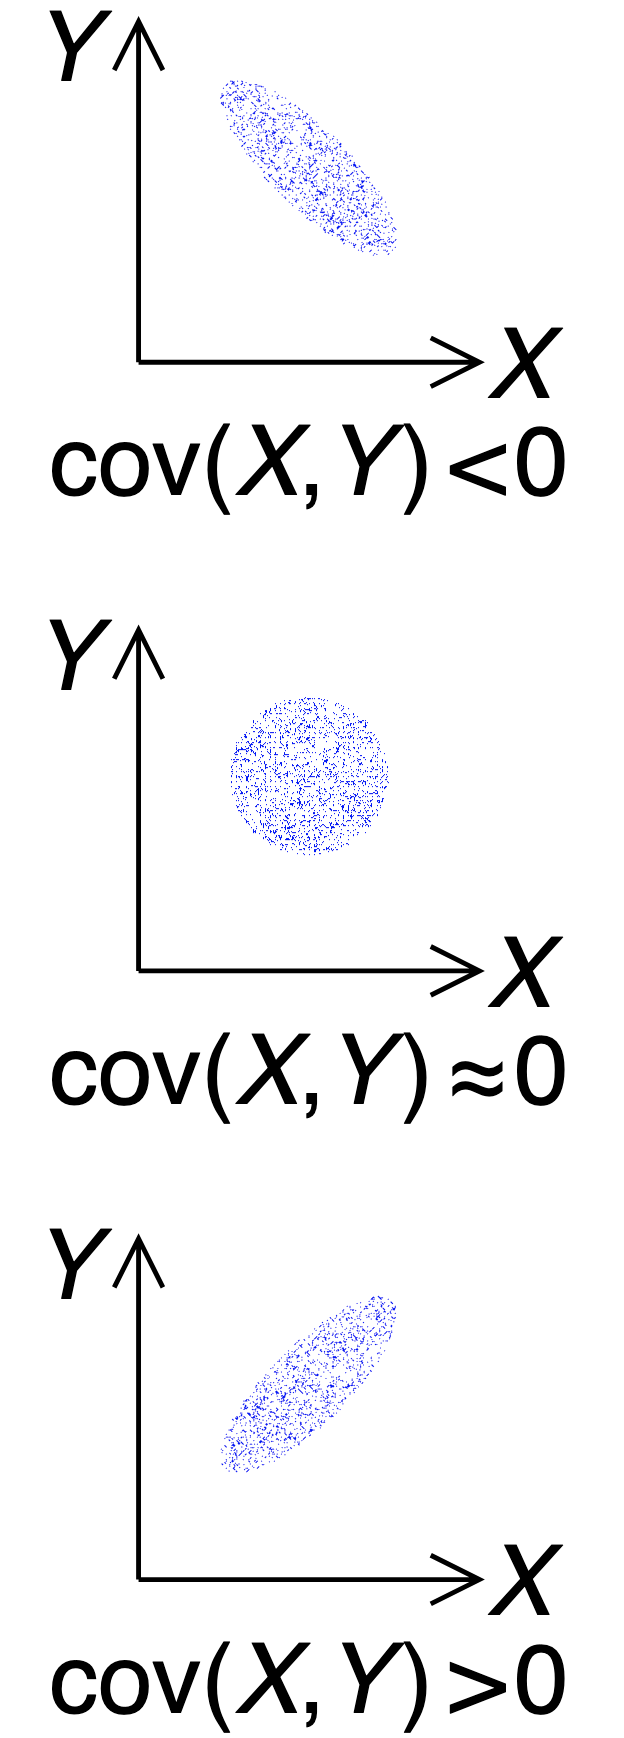
\includegraphics[scale=0.4]{img/cov_trends.png}
\end{figure}

\end{frame}


%%%%%%%%%%%%%%%%%%%%%%%%%%%%%%%%%%%%%%%%%%%%%%%%%%%%%%%%%%%%%%%%%%%%%%%%%%%%%%%%
\begin{frame}{Correlation}

The correlation of $X$ and $Y$ is defined by:
\begin{equation*}
    \rho_{X,Y} = \frac{\Cov{X, Y}}{\sigma_X \sigma_Y}
\end{equation*}
Notes:
\begin{itemize}
    \item Correlation is always between -1 and 1, with the values -1 and 1 indicating perfect linear relationships
\end{itemize}
\end{frame}



%%%%%%%%%%%%%%%%%%%%%%%%%%%%%%%%%%%%%%%%%%%%%%%%%%%%%%%%%%%%%%%%%%%%%%%%%%%%%%%%
\begin{frame}{Correlation coefficients}

\begin{figure}
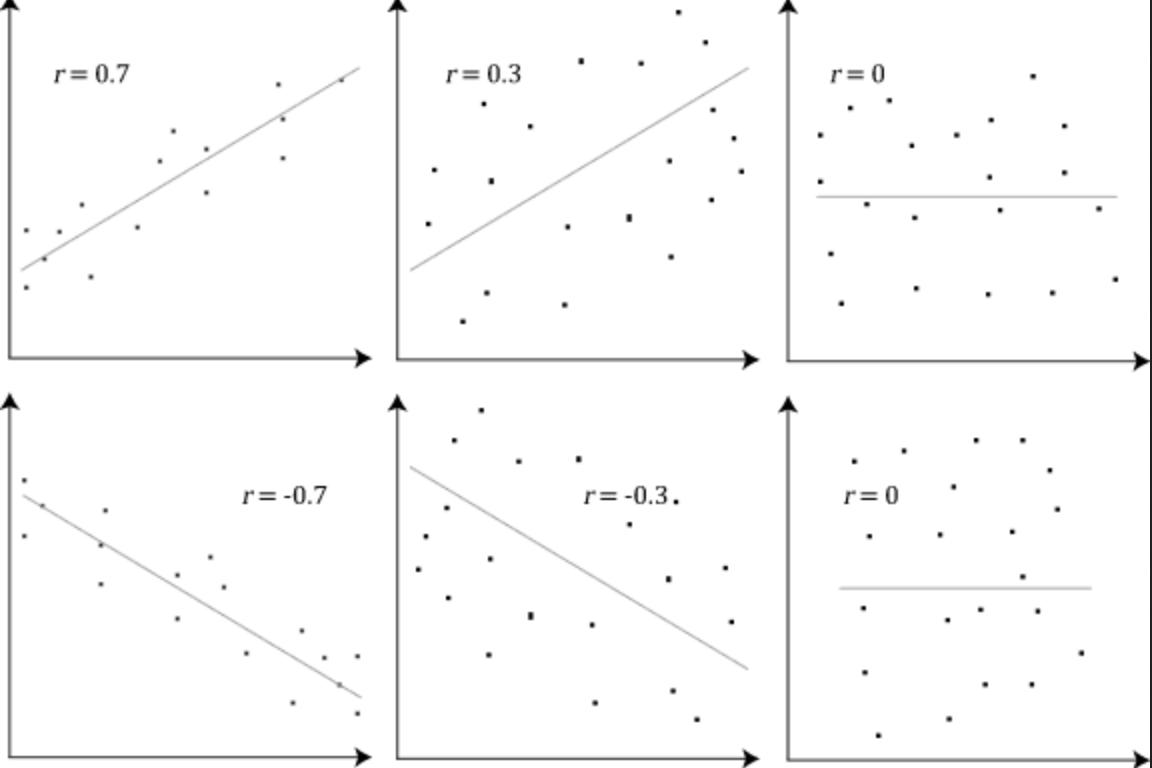
\includegraphics[scale=0.4]{img/correlation_coef.png}
\end{figure}

\end{frame}

%%%%%%%%%%%%%%%%%%%%%%%%%%%%%%%%%%%%%%%%%%%%%%%%%%%%%%%%%%%%%%%%%%%%%%%%%%%%%%%%
\begin{frame}{Covariance, correlation, and independence}

If $X$ and $Y$ are independent random variables, then $\Cov{X, Y} = 0$ and $\rho_{XY} = 0$
\begin{itemize}
    \item But the reverse is not necessarily true! You can have $\Cov{X, Y} = 0$, but $X$ and $Y$ are dependent!
    \item Covariance and correlation measure only a particular kind of linear relationship
\end{itemize}

\vspace{2ex}
\textbf{Example:} $X$ is uniform between $[-1, 1]$, and $Y=X^2$ (clearly depedendent!)
\begin{align*}
    \Cov{X, Y} =& \EE [XY] - \mu_X \mu_Y \\
    =& \EE [X \cdot X^2] - \EE [X] \cdot \EE [X^2] \\
    =& \EE [X^3] - 0 \cdot \EE [X^2] \\
    =& 0 - 0 = 0
\end{align*}

\end{frame}




% %%%%%%%%%%%%%%%%%%%%%%%%%%%%%%%%%%%%%%%%%%%%%%%%%%%%%%%%%%%%%%%%%%%%%%%%%%%%%%%%
% \begin{frame}{Law of large numbers}

% In this class, we will often deal with 


% \end{frame}

%%%%%%%%%%%%%%%%%%%%%%%%%%%%%%%%%%%%%%%%%%%%%%%%%%%%%%%%%%%%%%%%%%%%%%%%%%%%%%%%
\section[CEF]{Conditional Expectation Function (CEF)}
\miniframesoff
\begin{frame}
    \tableofcontents[currentsection]
\end{frame}
\miniframeson
%%%%%%%%%%%%%%%%%%%%%%%%%%%%%%%%%%%%%%%%%%%%%%%%%%%%%%%%%%%%%%%%%%%%%%%%%%%%%%%



%%%%%%%%%%%%%%%%%%%%%%%%%%%%%%%%%%%%%%%%%%%%%%%%%%%%%%%%%%%%%%%%%%%%%%%%%%%%%%%%
\begin{frame}{Conditional expectation}

Empirical economic research is often concerned with the statistical analysis of individual economic circumstances
\begin{itemize}
    \item Differences in economic fortune can be considered random
    \item In econometrics, we think we can summarize and interpret randomness in a useful way
\end{itemize}

\vspace{2ex}
\textbf{Example:} Connection between education and earnings
\begin{itemize}
    \item On average, people with more schooling earn more than people with less schooling
    \item There is clearly a predictive relationship between schooling and earnings
    \item \emph{But is this relationship causal?}
\end{itemize}

\vspace{2ex}
\textbf{Now:} we focus on the \textbf{predictive} relationship between variables
\begin{itemize}
    \item This is summarized by the conditional expectations function (CEF)
\end{itemize}
Reading: MHE 3.1: CEF and regression as predictive tools
\begin{itemize}
    \item MHE 3.2 moves on to regression and causality
\end{itemize}
\end{frame}

%%%%%%%%%%%%%%%%%%%%%%%%%%%%%%%%%%%%%%%%%%%%%%%%%%%%%%%%%%%%%%%%%%%%%%%%%%%%%%%%
\begin{frame}{CEF}

Say we have some \textbf{dependent variable} $Y_i$, and $K \times 1$ vector of covariates $\XX_i$ (with elements $X_{ki}$):
\begin{equation*}
\XX_i = \begin{bmatrix} X_{1i} \\ X_{2i} \\ \vdots \\ X_{ki} \\ \vdots \\ X_{Ki} \end{bmatrix}
\end{equation*}
The \textbf{conditional expectations function} (\textbf{CEF}) for a dependent variable $Y_i$ given $\XX_i$ is the expectation, or population average, of $Y_i$, with $\XX_i$ held fixed. 
\begin{equation*}
    \EE [Y_i \vert \XX_i]
\end{equation*}
To emphasize that the CEF is a function of $\XX$, we'll often write for some realized value $x$:
\begin{equation*}
    \EE [Y_i \vert \XX_i = x]
\end{equation*}
\textbf{Example}: Suppose $Y_i$ is earnings, and $D_i$ is whether an individual $i$ completed college. We can write:
\begin{equation*}
    \EE [Y_i \vert D_i = 0] \quad\quad \EE [Y_i \vert D_i = 1]
\end{equation*}
\end{frame}


%%%%%%%%%%%%%%%%%%%%%%%%%%%%%%%%%%%%%%%%%%%%%%%%%%%%%%%%%%%%%%%%%%%%%%%%%%%%%%%%
\begin{frame}{Discrete and continuous CEF}

Discrete CEF:
\begin{equation*}
    \EE [Y \vert X = x] = \sum_{y} y \PP (Y = y \vert X = x)
\end{equation*}
Continuous CEF: 
\begin{equation*}
    \EE [Y \vert X = x] = \int y f_Y (y \vert X = x) dy 
\end{equation*}

\end{frame}

%%%%%%%%%%%%%%%%%%%%%%%%%%%%%%%%%%%%%%%%%%%%%%%%%%%%%%%%%%%%%%%%%%%%%%%%%%%%%%%%
\begin{frame}{CEF example}

\begin{figure}
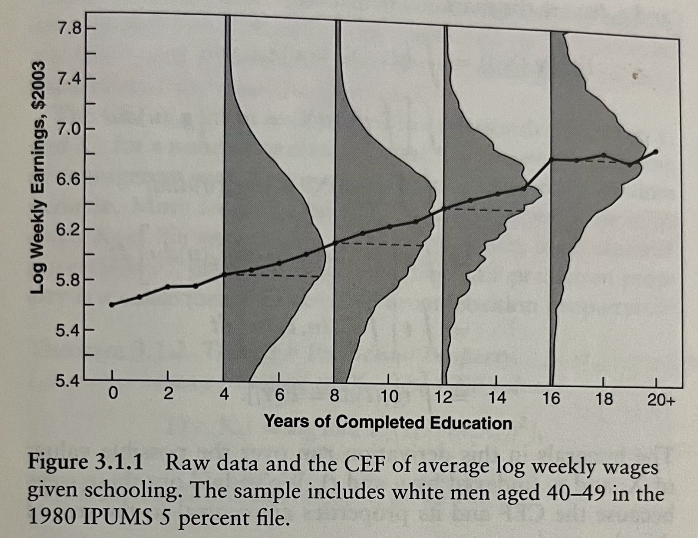
\includegraphics[scale=0.7]{img/CEF-example.png}
\end{figure}

\end{frame}

%%%%%%%%%%%%%%%%%%%%%%%%%%%%%%%%%%%%%%%%%%%%%%%%%%%%%%%%%%%%%%%%%%%%%%%%%%%%%%%%
\section[CEF Properties]{Properties of Conditional Expectation Function}
\miniframesoff
\begin{frame}
    \tableofcontents[currentsection]
\end{frame}
\miniframeson
%%%%%%%%%%%%%%%%%%%%%%%%%%%%%%%%%%%%%%%%%%%%%%%%%%%%%%%%%%%%%%%%%%%%%%%%%%%%%%%


%%%%%%%%%%%%%%%%%%%%%%%%%%%%%%%%%%%%%%%%%%%%%%%%%%%%%%%%%%%%%%%%%%%%%%%%%%%%%%%%
\begin{frame}{Law of Iterated Expectations (LIE)}

    Important property: 
    \begin{equation*}
    \EE [Y] = \EE_X \left[ \EE [Y \vert X] \right]
\end{equation*}

\vspace{2ex}
\textbf{Why is this important?} Suppose $Y$ denotes average earnings, and $X$ denotes gender (say $X=1$ is female). By LIE:
\begin{itemize}
    \item Find the average earnings for men in the population $\EE [Y \vert X = 0]$
    \item Find the average earnings for women in the population $\EE [Y \vert X = 1]$
    \item Find overall average earnings $\EE [Y]$ by taking the average for men times the proportion male in population, plus the average for women times the proportion female in the population
\end{itemize}

\end{frame}

%%%%%%%%%%%%%%%%%%%%%%%%%%%%%%%%%%%%%%%%%%%%%%%%%%%%%%%%%%%%%%%%%%%%%%%%%%%%%%%%
\begin{frame}{Law of Iterated Expectations - Proof}

\begin{equation*}
    \EE [Y] = \EE \left[ \EE [Y \vert X] \right]
\end{equation*}
Proof:
\begin{align*}
    \EE [Y] &= \sum_{j} y_j \PP (Y = y_j) \\
    \onslide<2->{&= \sum_{j} y_j {\color<2>{blue}\left(\sum_{i} \PP (Y = y_j, X = x_i)\right)} &\because\text{ marginalization }} \\
    \onslide<3->{
        &=\sum_{j} y_j \left(
            \sum_i {
            \color<3>{red} \PP (Y = y_j \vert X = x_i) \PP (X = x_i)
            }
        \right) &\because\text{Product Rule}
    } \\
    \onslide<4->{
        &= {\color<4>{blue} \sum_i } \left(
            \sum_j y_j \PP (Y = y_j \vert X = x_i)
        \right)
        {\color<4>{blue} \PP (X = x_i)}
    } \\
    \onslide<5->{
        &= \sum_i {\color<5>{red}
            \EE [Y \vert X = x_i]
        } \PP (X = x_i)
    } \\
    \onslide<6->{
        &= \EE_X [\EE [Y \vert X]]
    }
\end{align*}

\end{frame}

%%%%%%%%%%%%%%%%%%%%%%%%%%%%%%%%%%%%%%%%%%%%%%%%%%%%%%%%%%%%%%%%%%%%%%%%%%%%%%%%
\begin{frame}{LIE example}

\begin{table}
\begin{tabular}{ccc}
Student &Test number &Score \\
\hline\hline
$R$ &1 &95 \\
$R$ &2 &80 \\
\hline
$S$ &1 &100 \\
$S$ &2 &70
\end{tabular}
\end{table}

Note that: 
\begin{align*}
    \EE [\text{Score} \vert \text{Student} = R] &= \frac{95 + 80}{2} = \frac{175}{2} = 87.5 \\
    \EE [\text{Score} \vert \text{Student} = S] &= \frac{100 + 70}{2} = \frac{170}{2} = 85
\end{align*}
Using the law of iterated expectations:
\begin{align*}
    \EE [\text{Score}] &= \EE[ \EE[\text{Score} \vert \text{Student} ] ]\\
    &= \frac{87.5 + 85}{2} \\
    &= 86.25
\end{align*}

\end{frame}

%%%%%%%%%%%%%%%%%%%%%%%%%%%%%%%%%%%%%%%%%%%%%%%%%%%%%%%%%%%%%%%%%%%%%%%%%%%%%%%%
\begin{frame}{CEF Decomposition}

Any random variable $Y_i$ can be decomposed into the CEF plus a residual:
\begin{equation*}
    Y_i = 
    \underbrace{
        \EE [Y_i \vert X_i]
    }_{
        \onslide<2->{\text{Part of $Y_i$ explained by $X_i$}}
    } 
    + \underbrace{
        \epsilon_i
    }_{
        \onslide<2->{\text{Part of $Y_i$ \emph{not} explained by $X_i$}}
    }
\end{equation*}
where:
\begin{enumerate}
    \item $\epsilon_i$ is mean-independent of $X_i$ with mean zero, that is $\EE[\epsilon_i \vert X_i] = \EE [\epsilon_i] = 0$.
    \item $\epsilon_i$ is uncorrelated with any function of $X_i$
\end{enumerate}

\vspace{2ex}
\textbf{Why is this important?}
\begin{itemize}
    \onslide<2->{\item Allows us to breakdown $Y_i$ into part explained by $X_i$ and part \textbf{not} explained by $X_i$} 
    \onslide<2->{
        \item The leftover piece ($\epsilon_i$) is uncorrelated with \emph{any} function of $X_i$
        \begin{itemize}
            \item Unlike simple uncorrelatedness (only rules out linear patterns), this rules out \emph{any} systematic relationship between $\epsilon_i$ and $X_i$ - this is a stronger statement.
            \item We will see that this makes the CEF a very strong predictor
        \end{itemize}
        }
\end{itemize}


\end{frame}


%%%%%%%%%%%%%%%%%%%%%%%%%%%%%%%%%%%%%%%%%%%%%%%%%%%%%%%%%%%%%%%%%%%%%%%%%%%%%%%%
\begin{frame}{CEF Decomposition Proof}

Any random variable $Y_i$ can be decomposed into the CEF plus a residual:
\begin{equation*}
    Y_i = \EE [Y_i \vert X_i] + \epsilon_i
\end{equation*}
where $\epsilon_i$ is the part of $Y_i$ \emph{not} explained by $X_i$.

\vspace{2ex}
\textbf{Property (i):} $\epsilon_i$ is mean-independent of $X_i$:
\begin{equation*}
    \EE [\epsilon_i \vert X_i] = \EE [\epsilon_i] = 0
\end{equation*}

\textbf{Proof:}
\begin{align*}
    \epsilon_i &= Y_i - \EE [Y_i \vert X_i] \\
    \EE [\epsilon_i \vert X_i] &= \EE \left[ Y_i - \EE [Y_i \vert X_i] \; \vert \; X_i \right] \\
    &= \EE [Y_i \vert X_i] - \EE \left[ \EE [Y_i \vert X_i] \vert X_i \right] \\
    &= \EE [Y_i \vert X_i] - \EE [Y_i \vert X_i] = 0
\end{align*}
Then by the law of iterated expectations:
\begin{equation*}
    \EE [\epsilon_i] = \EE \left[ \EE [\epsilon_i \vert X_i] \right] = \EE [0] = 0
\end{equation*}

\end{frame}

%%%%%%%%%%%%%%%%%%%%%%%%%%%%%%%%%%%%%%%%%%%%%%%%%%%%%%%%%%%%%%%%%%%%%%%%%%%%%%%%
\begin{frame}{CEF Decomposition Proof (cont.)}

\textbf{Aside:} Two random variables are uncorrelated if $\Cov{X, Y} = 0$, i.e.\ $\EE [XY] = \EE [X] \EE [Y]$. If in addition $\EE [Y] = 0$, then for any function $h(X)$:
\begin{equation*}
    \EE [h(X) Y] = \EE [h(X)] \EE [Y] = 0
\end{equation*}

\vspace{2ex}
\textbf{Property (ii):} $\epsilon_i$ is uncorrelated with \emph{any} function of $X_i$. Let $h(X_i)$ be a function of $X_i$.

\vspace{1ex}
\textbf{Proof:} By the law of iterated expectations:
\begin{align*}
    \EE [h(X_i) \epsilon_i] &= \EE \left[ \EE [h(X_i) \epsilon_i \vert X_i] \right] \\
    &= \EE \left[ h(X_i) \EE [\epsilon_i \vert X_i] \right] \\
    &= \EE [h(X_i) \cdot 0] = 0
\end{align*}
Since $\epsilon_i$ is orthogonal to any function of $X_i$, the CEF decomposition splits $Y_i$ into the part explained by $X_i$ and a piece that is unrelated (in this strong sense) to $X_i$.

\end{frame}


%%%%%%%%%%%%%%%%%%%%%%%%%%%%%%%%%%%%%%%%%%%%%%%%%%%%%%%%%%%%%%%%%%%%%%%%%%%%%%%%
\begin{frame}{CEF Prediction Property}

Let $m(X_i)$ be any function of $X_i$. The conditional expectation function $\EE [Y_i \vert X_i]$ solves:
\begin{equation*}
    \EE [Y_i \vert X_i] = \argmin_{m(X_i)} \; \EE \left[ (Y_i - m(X_i))^2 \right]
\end{equation*}
$\implies$ the CEF is the \textbf{minimum mean squared error (MSE) predictor} of $Y_i$ given $X_i$:

\vspace{2ex}
\textbf{Why is this important?}
\begin{itemize}
    \item The CEF $\EE [Y_i \vert X_i]$ is a type of \textbf{prediction rule}, where you generate predictions of $Y_i$ as a function of $X_i$. One could use other prediction rules $m(X_i)$ to predict $Y_i$.
    \item The Mean Squared Error (MSE) is a way of evaluating the difference between predicted $Y_i$ and true $Y_i$. 
    \item Because the CEF solves the minimum mean squared error prediction problem, the CEF Prediction is the best predictor of $Y_i$ given $X_i$, in a mean squared sense. 
\end{itemize}

\end{frame}

%%%%%%%%%%%%%%%%%%%%%%%%%%%%%%%%%%%%%%%%%%%%%%%%%%%%%%%%%%%%%%%%%%%%%%%%%%%%%%%%
\begin{frame}{CEF Prediction Property Proof}

Let $m(X_i)$ be any function of $X_i$. The CEF solves:
\begin{equation*}
    \EE [Y_i \vert X_i] = \argmin_{m(X_i)} \; \EE \left[ (Y_i - m(X_i))^2 \right]
\end{equation*}
$\implies$ the CEF is the \textbf{minimum mean squared error (MSE) predictor} of $Y_i$ given $X_i$:
% \begin{itemize}
%     \item It provides a representative value of $Y_i$ given $X_i$
%     \item It solves the minimum mean squared error prediction problem
% \end{itemize}

\vspace{1ex}
\textbf{Proof:} Add and subtract $\EE [Y_i \vert X_i]$, then expand:
\begin{align*}
    (Y_i - m(X_i))^2 
    =& \left( 
        Y_i - \EE [Y_i \vert X_i]
        + \EE [Y_i \vert X_i] - m(X_i)
        \right)^2 \\
    =& \left( 
        {\color{MainBlue}(Y_i - \EE [Y_i \vert X_i])} 
        + {\color{Green} (\EE [Y_i \vert X_i] - m(X_i))} 
       g \right)^2 \\
    =& 
        {\color{MainBlue}(Y_i - \EE [Y_i \vert X_i])}^2 
        + 2 \underbrace{{\color{MainBlue}(Y_i - \EE [Y_i \vert X_i])}}_{\epsilon_i} 
        \underbrace{{\color{Green} (\EE [Y_i \vert X_i] - m(X_i))}}_{h(X_i)}
        \\ &\quad + {\color{Green} (\EE [Y_i \vert X_i] - m(X_i))}^2 \\
    =& 
        {\color{MainBlue}(Y_i - \EE [Y_i \vert X_i])}^2 
        + 2 {\color{MainBlue}\epsilon_i} 
        {\color{Green} h(X_i)}
        + {\color{Green} (\EE [Y_i \vert X_i] - m(X_i))}^2
\end{align*}
Taking expectations, the cross term vanishes since $\EE [h(X_i) \epsilon_i] = 0$ (Property ii):
\begin{equation*}
    \EE \left[ (Y_i - m(X_i))^2 \right] = \underbrace{\EE \left[ (Y_i - \EE [Y_i \vert X_i])^2 \right]}_{\text{does not involve } m(X_i)} + \underbrace{\EE \left[ (\EE [Y_i \vert X_i] - m(X_i))^2 \right]}_{\text{minimized at } m(X_i) = \EE [Y_i \vert X_i]}
\end{equation*}

\end{frame}

%%%%%%%%%%%%%%%%%%%%%%%%%%%%%%%%%%%%%%%%%%%%%%%%%%%%%%%%%%%%%%%%%%%%%%%%%%%%%%%%
\begin{frame}{ANOVA Theorem}

The variance of $Y_i$ decomposes as:
\begin{equation*}
    \Var{Y_i} = \Var{\EE [Y_i \vert X_i]} + \EE \left[ \Var{Y_i \vert X_i} \right]
\end{equation*}

\vspace{1ex}
\textbf{Why is this useful?}
\begin{itemize}
    \item Decompositions are helpful tools for summarizing data
    \item They work in the population as well as in a sample
    \item They do not rely on any linearity assumption on the CEF
\end{itemize}

\end{frame}

%%%%%%%%%%%%%%%%%%%%%%%%%%%%%%%%%%%%%%%%%%%%%%%%%%%%%%%%%%%%%%%%%%%%%%%%%%%%%%%%
\begin{frame}{ANOVA Theorem (Proof)}

\textbf{Proof:} From the CEF decomposition, $Y_i = \EE [Y_i \vert X_i] + \epsilon_i$, so:
\begin{align*}
    \Var{Y_i} &= \Var{\EE [Y_i \vert X_i] + \epsilon_i}
\end{align*}
For any two random variables $A$ and $B$:
\begin{align*}
    \Var{A + B} &= \Var{A} + \Var{B} + 2 \Cov{A, B}
\end{align*}
Applying this to the CEF decomposition: 
\begin{align*}
    \Var{Y_i} &= \Var{\EE [Y_i \vert X_i] + \epsilon_i} \\
    &= \Var{\EE [Y_i \vert X_i]} + \Var{\epsilon_i} + 2 \Cov{\EE [Y_i \vert X_i], \epsilon_i} \\
    &= \Var{\EE [Y_i \vert X_i]} + \Var{\epsilon_i}
\end{align*}
Since $\EE [\epsilon_i] = 0$, $\Var{\epsilon_i} = \EE [\epsilon_i^2]$. By the law of iterated expectations:
\begin{align*}
    \EE [\epsilon_i^2] &= \EE \left[ \EE [\epsilon_i^2 \vert X_i] \right] = \EE \left[ \EE \left[ (Y_i - \EE [Y_i \vert X_i])^2 \vert X_i \right] \right] = \EE \left[ \Var{Y_i \vert X_i} \right]
\end{align*}
so:
\begin{equation*}
    \Var{Y_i} = \Var{\EE [Y_i \vert X_i]} + \EE \left[ \Var{Y_i \vert X_i} \right]
\end{equation*}



\end{frame}


\end{document}





